
\section{User Interface}
\label{sec:demo}


To demonstrate \system's exploratory search we loaded scientific 
papers from the DBLP conference~\cite{Tang:2008:EMA:1367497.1367722} 
and also Wikipedia articles downloaded using the MediaWiki API~\footnote{\texttt{https://www.mediawiki.org}}.
The {\system} website has a list of topics with a slider associated 
with each of them using which a user can specify the degree of 
interest in that particular topic. The weightage specified by each 
slider corresponds to the components of the user model. The user 
model is a profile of preference provided by the user before she 
makes any search.

Initially, all the extracted topics from the corpus are shown along 
with their most informative words (see Figure~\ref{fig:topic_exploration}).
This list is color coded to distinguish the relevance of topics as indicated by the user model --- much like a heat map.
The user can look at this heat map to adjust their topic preferences.
The list is clickable and once a topic is selected, relevant articles to that topic ranked based on the user model are displayed.
%We use Equation~\ref{eq:KL} to calculate this preference on the \system browser. 
In the \textsl{Graph Explorer} interface, the citations for the current article is ranked
using Equation~\ref{eq:KL}. The citations (of that article) that are most
similar to the user model are ranked the highest.
%A screenshot is shown in Figure~\ref{fig:topic_exploration}.


%\paragraph{Keyword Paper Explore}
The tab \textsl{Keyword Paper Search} (Figure~\ref{fig:topic_exploration}) contains the interface for the user model weighted keyword search.
The user may enter one or more keywords representing topics,  
author names, etc. The keywords are searched in the title, abstract, 
and author fields of all the articles. The discovered results are  
re-weighted using the user model. 
\eat{
In the first page only a few of 
the articles are displayed in two boxes --- one containing matching words in the title, and the other in the abstract.
Clicking on any box will open up a more complete list of articles.}

\begin{figure}[htb]\centering
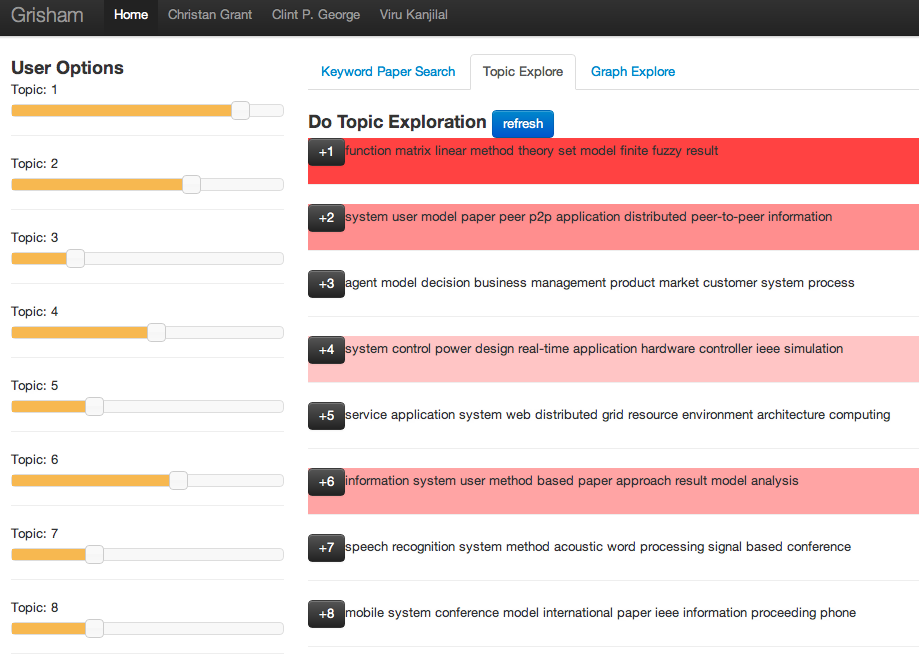
\includegraphics[width=.45\textwidth]{images/topic_exploration.png} % scale=.25,trim=0 0 300 0
\caption{The interface for examining the effect of changes to the user model on the topics.}
\label{fig:topic_exploration}
\end{figure}

For topic exploration \system allows a user to click on a specific 
topic to see the informative words for that topic in a word cloud 
(Figure~\ref{fig:topic-word-cloud}). By selecting a topic the user 
can explore more about the articles associated with the topic using 
Force-Directed Graph~\cite{2011-d3} (Figure~\ref{fig:topic-search-viz}).
A user can navigate to a particular document by clicking a document 
node (orange) in the graph. 

On the document visualization page, we show a doughnut chart for the document topic distribution as well as a preview of the document contents.
Clicking on the topics in the doughnut chart will take the user to the topic word cloud page.
Selecting a section or paragraph changes the doughnut chart to reflect the topic distribution specific to that selection.
For example, the document visualization page for \textit{Killer whale} is displayed in Figure~\ref{fig:doc-para-viz}.





\begin{figure}[htb]\centering 
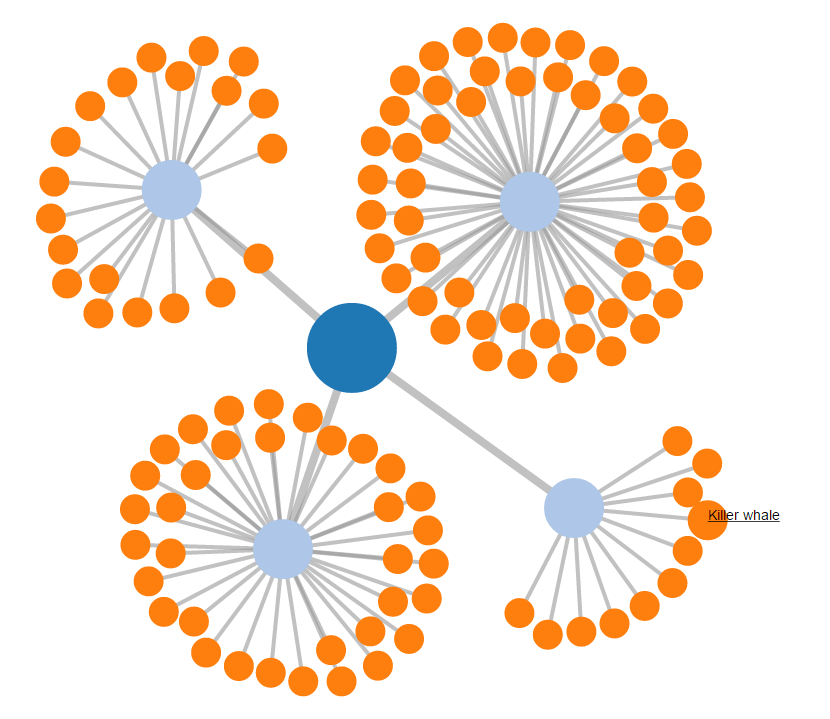
\includegraphics[width=.5\textwidth]{images/topical_docs.png}
\caption{Visualizing \textsl{topic-based search} in \system, orange 
nodes represent documents and blue nodes represent the estimated 
topics in a corpus. For this illustration we only show four topics 
(light blue nodes). Topic names appear when the user hovers over a 
node.}
\label{fig:topic-search-viz}
\end{figure}

\begin{figure*}[htb]\centering 
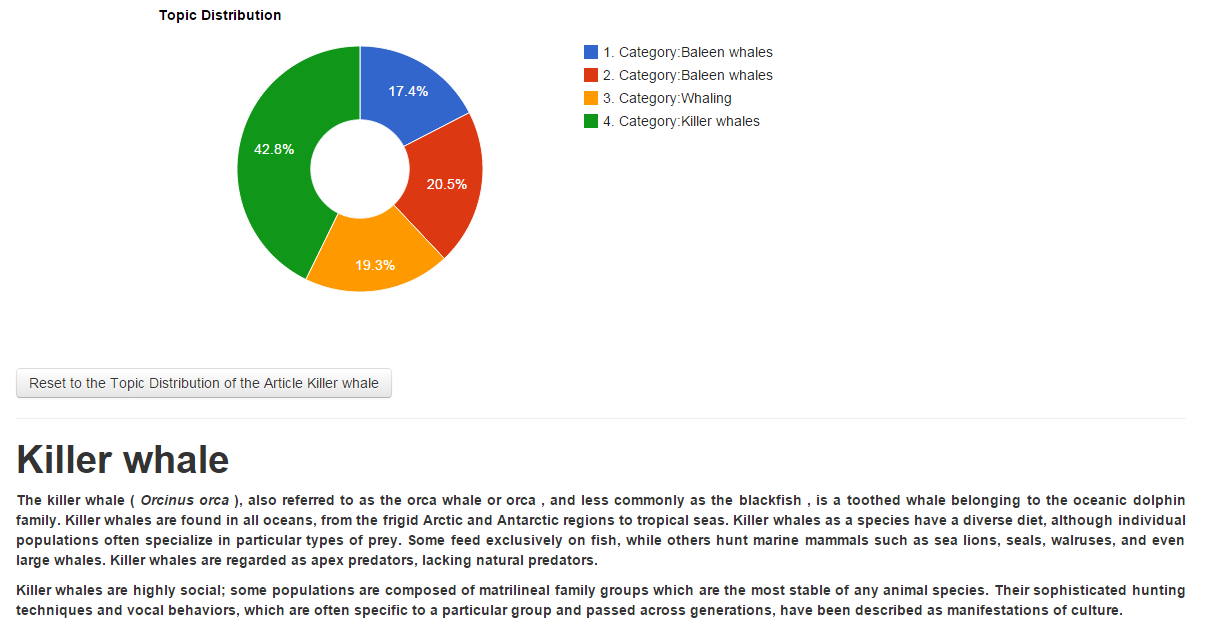
\includegraphics[width=1\textwidth]{images/para_topic_distribution.png}
\caption{Visualizing the topic distribution of the introduction 
section of the Wikipedia article \textit{Killer Whale}. See Figure~\ref{fig:doc-topic-distribution} for the topic distribution of 
the whole article.}
\label{fig:doc-para-viz}
\end{figure*}

\eat{
\begin{figure}[htb]\centering 
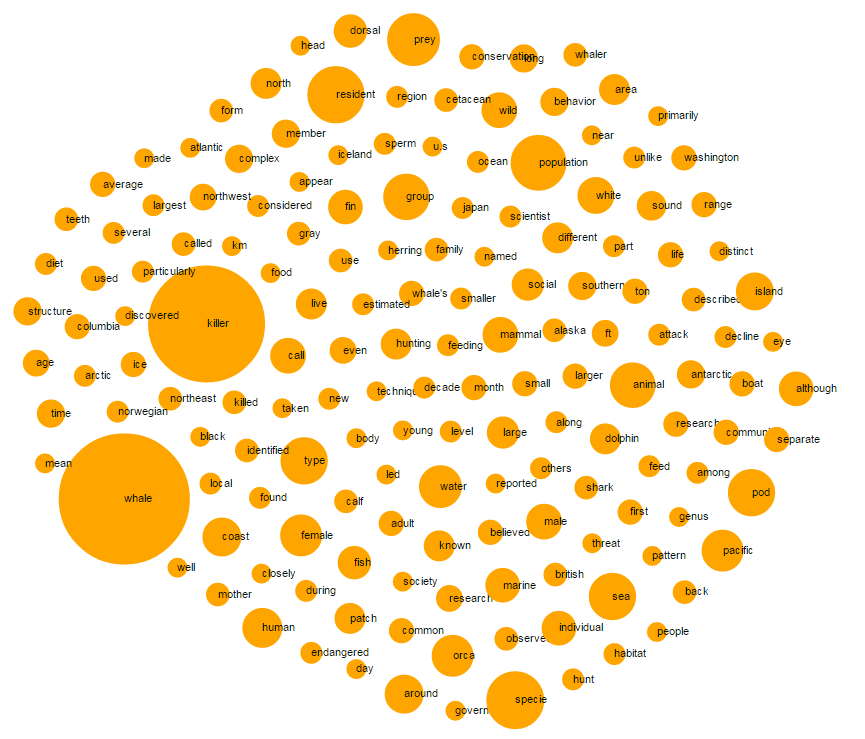
\includegraphics[width=.5\textwidth]{images/doc_tf_bubble_chart.png}
\caption{Visualizing the relative frequencies of terms in the 
Wikipedia article \textit{Killer Whale}. \cpg{I think we need to 
decide whether we should keep this figure in the paper or not.}}
\label{fig:doc-word-counts}
\end{figure}
}

% \paragraph{Graph Explore}
%One of the most interesting visualizations in the project is the 
%\textsl{Graph Explore} interface which 

The \textsl{Graph Explore} interface allows a user to recursively 
drill down a graph of an article and its out-links (citations).
This is a common method of literature exploration; a user takes up a base article and then reads up all the articles which have been cited in that base article.
These steps are recursively performed for each subsequent article until the user has found a sufficient amount of articles or they have read all the articles in their collection.
%Though effective, this technique tell the user which ones he should pursue and which ones he should now.
The graph explore interface allows a user to perform this in a more visually appealing manner.
Once a user decides on a base article (through any search scheme), the system shows a graph representation of its citations which are ranked based on her profile (i.e. \textsl{user model}).
This will help her pursue the most relevant articles first.
Clicking on any secondary article will expand the graph further and 
list secondary citations ranked based on the \textsl{user model}.
